	%
% Niniejszy plik stanowi przykład formatowania pracy magisterskiej na
% Wydziale MIM UW.  Szkielet użytych poleceń można wykorzystywać do
% woli, np. formatujac wlasna prace.
%
% Zawartosc merytoryczna stanowi oryginalnosiagniecie
% naukowosciowe Marcina Wolinskiego.  Wszelkie prawa zastrzeżone.
%
% Copyright (c) 2001 by Marcin Woliński <M.Wolinski@gust.org.pl>
% Poprawki spowodowane zmianami przepisów - Marcin Szczuka, 1.10.2004
% Poprawki spowodowane zmianami przepisow i ujednolicenie 
% - Seweryn Karłowicz, 05.05.2006
% Dodanie wielu autorów i tłumaczenia na angielski - Kuba Pochrybniak, 29.11.2016

% dodaj opcję [licencjacka] dla pracy licencjackiej
% dodaj opcję [en] dla wersji angielskiej (mogą być obie: [licencjacka,en])
\documentclass[licencjacka]{pracamgr}

% Dane magistrantów:
\autor{Maciej Góralski}{346144
\vspace{2em}}
\autori{Kacper Pawelec}{332436
\vspace{2em}}
\autorii{Aliaksei Suvorau}{374118}
\autoriii{Michał Swidziński}{371800}


% Dane magistrantów:
%\autor{Autor Zerowy}{342007}
%\autori{Autor Pierwszy}{342013}
%\autorii{Drugi Autor-Z-Rzędu}{231023}
%\autoriii{Trzeci z Autorów}{777321}
%\autoriv{Autor nr Cztery}{432145}
%\autorv{Autor nr Pięć}{342011}

\title{Zapisy na spotkania w systemie USOS}


%\tytulang{An implementation of a difference blabalizer based on the theory of $\sigma$ -- $\rho$ phetors}

%kierunek: 
% - matematyka, informacyka, ...
% - Mathematics, Computer Science, ...
\kierunek{informatyka}

% informatyka - nie okreslamy zakresu (opcja zakomentowana)
% matematyka - zakres moze pozostac nieokreslony,
% a jesli ma byc okreslony dla pracy mgr,
% to przyjmuje jedna z wartosci:
% {metod matematycznych w finansach}
% {metod matematycznych w ubezpieczeniach}
% {matematyki stosowanej}
% {nauczania matematyki}
% Dla pracy licencjackiej mamy natomiast
% mozliwosc wpisania takiej wartosci zakresu:
% {Jednoczesnych Studiow Ekonomiczno--Matematycznych}

% \zakres{Tu wpisac, jesli trzeba, jedna z opcji podanych wyzej}

% Praca wykonana pod kierunkiem:
% (podać tytuł/stopień imię i nazwisko opiekuna
% Instytut
% ew. Wydział ew. Uczelnia (jeżeli nie MIM UW))
\opiekun{dr Janina Mincer-Daszkiewicz\\
  Uniwersytet Warszawski\\
  }

% miesiąc i~rok:
\date{Grudzień 2018}

%Podać dziedzinę wg klasyfikacji Socrates-Erasmus:
\dziedzina{ 
%11.0 Matematyka, Informatyka:\\ 
%11.1 Matematyka\\ 
%11.2 Statystyka\\ 
11.3 Informatyka\\ 
%11.4 Sztuczna inteligencja\\ 
%11.5 Nauki aktuarialne\\
%11.9 Inne nauki matematyczne i informatyczne
}

%Klasyfikacja tematyczna wedlug AMS (matematyka) lub ACM (informatyka)
\klasyfikacja{Software and its engineering\\
Software creation and management\\
Software evolution\\}

% Słowa kluczowe:

\keywords{USOS, USOSadm, USOSweb, zapisy, spotkania, Dziekan, Sekcja Studencka}

% Tu jest dobre miejsce na Twoje własne makra i~środowiska:
\newtheorem{defi}{Definicja}[section]
\usepackage{hyperref}
\usepackage{enumitem}
\usepackage{calc}
\usepackage{tabularx}
\usepackage{array}
\usepackage{booktabs}
\usepackage[tableposition = top]{caption}
% \usepackage[none]{hyphenat}
\usepackage{graphicx}

\newlist{step}{enumerate}{10}
\setlist[step]{label*=\arabic*.,leftmargin=2em}
%\setlistdepth{10}

\newcolumntype{s}{>{\hsize=.35\hsize}X}
\newcolumntype{h}{>{\centering}X}
\newcolumntype{v}{>{\hsize=28px\centering\arraybackslash}X}
\newcolumntype{m}{>{\hsize=50px\centering\arraybackslash}X}
\newcolumntype{n}{>{\hsize=50px\arraybackslash}X}

\usepackage{csquotes}
\DeclareQuoteAlias{dutch}{polish}

% koniec definicji

\begin{document}

\maketitle

%tu idzie streszczenie na strone poczatkowa
\begin{abstract}
  Praca polega na dodaniu funkcjonalności do systemów USOSadm i USOSweb.
  Funkcjonalność ta umożliwi zdalną rejestrację zapisów do Dziekana dla studentów, co zaoszczędzi czasu, zmniejszy kolejki do Sekcji Studenckiej i pozwoli na zbieranie informacji do celów statystycznych.
  Ponadto zdalna rejestracja będzie dużo wygodniejsza zarówno dla Dziekana, pracowników Sekcji Studenckiej jak i studentów.
\end{abstract}

\tableofcontents
%\listoffigures
%\listoftables

\chapter{Wprowadzenie} \label{chap:wpr}
\section{Spotkanie}
Niektóre problemy wymagają osobistego spotkania z Dziekanem Wydziału Matematyki, Informatyki i Mechaniki Uniwersytetu Warszawskiego (MIM). Niniejsza praca ma na celu usprawnienie procesu zapisów na spotkanie z Dziekanem.
\section{Rozwiązanie dotychczasowe}
Obecnie student chcący zapisać się na spotkanie z Dziekanem MIM musi przejść przez następujący proces:
\begin{enumerate}
\item przyjść, zadzwonić albo wysłać wiadomość e-mail do Sekcji Studenckiej (Dziekanatu),
\item podać imię, nazwisko, numer indeksu oraz powód wizyty,
\item student otrzymuję odpowiedź od Sekcji Studenckiej. W przypadku kiedy problem wymaga spotkania z Dziekanem otrzymuje datę wizyty oraz numer w kolejce na liście wizyt. W przypadku, kiedy problem może być rozwiązany inaczej otrzymuje instrukcje, co powinien zrobić.
\end{enumerate}
Studenci preferują zapisywanie się osobiście, ponieważ natychmiast otrzymują pewną odpowiedź. Wizyty w Sekcji Studenckiej wymagają od studenta poświęcenia czasu i dostosowania się do krótkiego czasu pracy Sekcji. Przykładowym okresem, gdy szczególnie trudno jest uzyskać kontakt z~Sekcją~Studencką, jest okres przedłużania ważności legitymacji studenckich. Wtedy kolejki studentów potrafią być na tyle długie, że w rozsądnym czasie student nie będzie mógł wejść do~sekretariatu. Istnieje zapotrzebowanie na zmniejszenie tłoku w Sekcji Studenckiej.

Kluczowy jest tutaj fakt, że Sekcja Studencka na Wydziale MIM otwarta jest dla studentów tylko w poniedziałki, wtorki, czwartki i~piątki przez okres 3 godzin dziennie. Ogranicza to czasowe możliwości studentów na zapisy. Co więcej, forma, w jakiej przebiegają zapisy, niepotrzebnie zajmuje czas studentów i~pracowników Sekcji Studenckiej.

Ponadto różne sposoby kontaktu mogą powodować niesprawiedliwą kolejność wizyt.


\section{Ogólnie informacje o systemie USOS}
\href{http://usos.edu.pl}{USOS}, czyli Uniwersytecki System Obsługi Studiów, powstał w~wyniku zapotrzebowania na~narzędzie~informatyczne służące do~zarządzania sprawami studiów na~polskich~uczelniach. Razem z~sukcesem USOS powstała potrzeba,żeby stworzyć platformę umożliwiającą studentom częściowy dostęp do możliwości jakie dostarcza USOS. W tym celu powstał \href{htpp://usosweb.uw.edu.pl}{USOSweb}, czyli Internetowa platforma pozwalająca studentom i pracownikom uczelni na dostęp do części funkcjonalności USOS.

USOS dostarcza między innymi takie usługi jak:
\begin{enumerate}
\item rekrutacja na studia i~immatrykulacja,
\item elektroniczne Legitymacje Studenckie,
\item przygotowywanie oferty dydaktycznej,
\item zarządzanie tokiem studiów,
\item podania, stypendia i~ankiety,
\item akademiki i~płatności.
\end{enumerate}

USOS składa się między innymi z:
\begin{itemize}
\item USOSadm w Javie -- moduł przeznaczony dla pracowników administracji, pozwalający na cyfryzację typowych zadań administracyjnych, jak zarządzanie rejestracjami, płatnościami, wymianą międzynarodową i tym podobne,
\item USOSWeb -- moduł przeznaczony dla studentów napisany w PHP, udostępnia podstawowe informacje o~toku~studiów studenta oraz~funkcje~zdalnego załatwiania wielu formalności, jak rejestracja na przedmioty czy składanie podań.
\end{itemize}


\section{Cel pracy}
W ramach pracy powstał moduł do systemów USOSadm i~USOSweb, dzięki któremu będzie możliwe umawianie, kontrola i~archiwizacja wizyt studentów u~Dziekana. W USOSweb studenci i~osoby spoza wydziału będą mogły zapisywać się na spotkania z~Dziekanem w~odgórnie ustalonych terminach. Poza ułatwieniem rejestracji i~zwiększeniem jej dostępności, system ten będzie oszczędzać czas Dziekana oraz studentów. Ponadto zmniejszy się zużycie papieru.
\section{Struktura pracy}
Praca składa się z~6 rozdziałów i~dodatków.
Wymagania i~uwagi potencjalnych użytkowników zostały opisane w~rozdziale~\ref{chap:wymagania}.
W~rozdziale~\ref{chap:specyfikacja} znajduje się specyfikacja nowych funkcjonalności. W~rozdziale \ref{chap:implementacja} jest zawarty opis technologii użytych do~implementacji oraz jej szczegóły. Potencjalny dalszy rozwój nowego modułu jest opisany w~rozdziale \ref{chap:rozwoj}, a dokumentacje dotyczące wytworzonej w ramach niniejszej pracy funkcjonalności są w~rozdziale~\ref{chap:dodatki}. 

\section{Podział pracy}
\subsection{Maciej Góralski}
Napisał większość pracy licencjackiej.
\subsection{Kacper Pawelec}
Stworzył widoki słownik uzasadnień, kalendarz w USOSadm.
\subsection{Aliaksei Suvorau}
Zaprojektował bazę danych, napisał skrypt tworzący bazę danych Oracle. Zaimplementował wszystkie funkcje USOSweb.
\subsection{Michał Swidziński}
Napisał skrypt tworzący bazę danych MySQL. Stworzył widok notatki w USOSadm. Napisał część pracy licencjackiej.


\chapter{Wymagania użytkowników} \label{chap:wymagania}

\section{Wymagania}
Przed przystąpieniem do projektowania systemu postanowiliśmy zapytać potencjalnych użytkowników jakie mają wymagania względem systemu. Zidentyfikowaliśmy trzy główne grupy użytkowników które zapytaliśmy o zdanie: Dziekana, studentów oraz~pracowników Sekcji Studenckiej Dziekanatu.

\section{Rozmowa z Dziekanem}
Dziekana, będącego jednym z głównych odbiorców modułu, jako pierwszego zapytaliśmy o~wymagania względem projektu. Najistotniejsze z~nich to:

\begin{itemize}
\setlength\itemsep{0,1em}
\item powinien istnieć mechanizm ręcznej i automatycznej akceptacji próśb o spotkanie,
\item moduł musi dawać możliwość konfiguracji limitów czasowych oraz limitów ilości osób,
\item jak najwięcej pól w widokach spraw dla Dziekana oraz Sekcji powinno mieć domyślnie wypełnione wartości w celu przyśpieszenia pracy,
\item proces zapisywania się do Dziekana nie powinien być łatwy (np. trzeba szczegółowo opisać temat wizyty),
\item jednocześnie można być zapisanym tylko na jedno spotkanie,
\item Dziekan powinien mieć możliwość zostawienia w systemie notatki ze~spotkania,
\item system powinien być zaprojektowany w sposób, umożliwiający łatwe usuwanie większości informacji oraz zachowanie ważnych informacji archiwalnych (np. notatki i daty spotkań).
\end{itemize}
Wymagania jakie przedstawił Dziekan w dużej mierze uformowały kształt, jaki ten projekt przyjął. Na ich podstawie rozwijaliśmy lub~dodawaliśmy do modułu funkcjonalności.

\section{Ankieta dla studentów} \label{sec:ankieta}
W trakcie projektowania modułu przeprowadziliśmy ankietę internetową wśród studentów MIM, aby dowiedzieć się, jakie byłyby ich preferencje względem niektórych funkcjonalności i~czy pokrywają się z~wymyślonymi przez nas rozwiązaniami. Ankietę wypełniło 170 studentów. Poniżej zaprezentowano pytania i odpowiedzi.
\begin{itemize}
\setlength\itemsep{0,1em}
\item Jak wcześnie przed wizytą chciałbyś/chciałabyś zapisać się do dziekana?
Odpowiedziało 169 studentów.
\begin{itemize}
\setlength\itemsep{0,1em}
\item Tego samego dnia - 17 (28\%).
\item Na tydzień przed - 113 (67\%).
\item Na dwa tygodnie przed - 5 (3\%).
\item Na trzy tygodnie przed - 0.
\item Na miesiąc przed - 3 (2\%).
\item Na dłużej niż miesiąc przed - 0.
\end{itemize}

\item W wypadku gdy limit dostępnych miejsc się zapełni, chciałbyś/chciałabyś?
Odpowiedziało 170 studentów.
\begin{itemize}
\setlength\itemsep{0,1em}
\item Zostać zapisanym/zapisaną na najbliższy dostępny termin - 17 (10\%).
\item Zostać zapisanym na następny termin wyznaczony przez siebie - 135 (79\%).
\item Nic, chcę zapisać się od nowa samodzielnie - 18 (11\%).
\end{itemize}

\item Podając powód na wizytę u Dziekana, chcę.
Odpowiedziało 170 studentów.
\begin{itemize}
\setlength\itemsep{0,1em}

\item Napisać powód samemu - 11 (6\%).
\item Wybrać powód z listy dostępnych możliwych powodów - 16 (9\%).
\item Mieszankę powyższych odpowiedzi - 143 (84\%).
\end{itemize}

\item Czy zapisując się do Dziekana bierzesz pod uwagę sytuację, gdy nie będziesz w stanie pojawić się na wizycie?
Odpowiedziało 168 studentów.
\begin{itemize}
\setlength\itemsep{0,1em}

\item tak - 51 (30\%).
\item nie - 117 (70\%).
\end{itemize}

\item Jeśli tak, to z jakiego powodu i z jakim wyprzedzeniem przed wizytą będziesz o tym wiedzieć?
Odpowiedziało 44 studentów. Poniżej przytoczono niektóre odpowiedzi (tekst i pisownia oryginalne).
\begin{itemize}
\setlength\itemsep{0,1em}
\item \enquote{Chcę móc odwołać bez podania powodu}
\item \enquote{Zazwyczaj z powodu nagłych wypadków / choroby - 1-4 dni przed / rano tego samego dnia}
\item \enquote{wypadki losowe, 2-3 dni przed}
\item \enquote{24h brzmi sensownie}
\item \enquote{choroba, samodzielne rozwiązanie problemu przed wizytą, poprzedniego dnia}
\end{itemize}

\item Dodatkowe uwagi. Jeśli masz pomysł na wygodny dla studenta i akceptowalny przez dziekana sposób zapisów, to go opisz. Pamiętaj, że system zapisów musi być odporny na: niepotrzebne rezerwowanie wielu miejsc przez jedną osobę, \enquote{okienka} w grafiku dziekana, generowanie zbędnego ruchu w USOSweb, wymóg wielokrotnego zaglądania do USOSweb przez studenta w celu sprawdzenia, czy zapisy zakończy się sukcesem.
Odpowiedziało 31 studentów. Poniżej przytoczono niektóre odpowiedzi (tekst i pisownia oryginalne).
\begin{itemize}
\setlength\itemsep{0,1em}
\item \enquote{Odnośnie pytania "Z jakim wyprzedzeniem przed wizytą chciałbyś/chciałabyś zapisać się do dziekana?":    Chciałbym wybrać opcję "na dzień przed". Nie było takiej, więc wybrałem "tego samego dnia".}
\item \enquote{Fajnie byłoby widzieć o której godzinie trzeba przyjść, a nie tylko wiedzieć ze jest się 20 na liście.}
\item \enquote{Moim zdaniem, byłoby wspaniale, gdyby osoba1 mogła w ciągu tygodnia przed wizytą wypisać się z listy, a na jej miejsce mogłaby dopisać się osoba2, która próbowała dostać się w tym terminie ale limit miejsc był już zapełniony (na przykład osoba2 mogłaby dostawać maila, że miejsce zostało zwolnione i można dopisać się).}
\item \enquote{Ad pytanie 1 -- 3-5 dni przed    Ad pytanie 2 -- chciałbym zobaczyć, jakie są najbliższe wolne terminy i wybrać któryś z nich jeśli pasuje. Zapisywanie na najbliższy z automatu jest bez sensu, bo może nie pasować). Przy braku terminów, lub zapisie na dalszy niż pożądany, można by dodać opcję "powiadom mnie, jeśli zwolni się wcześniejszy termin". Po zwolnieniu terminu system mógłby wysłać powiadomienie mailem do kilku pierwszych osób z kolejki, można by wtedy przełożyć termin swojego spotkania na zwolniony -- na zasadzie "kto pierwszy ten lepszy", w szczególności, kto kliknie w powiadomienie jako drugi zawsze może zająć poprzedni termin tego kto kliknął pierwszy :)    Ad pytanie 3 -- najsensowniejszą opcją wydaje mi się połączenie    (1) wybór kategorii wizyty z listy ustalanej (i konfigurowalnej) przez Dziekana (tak żeby ułatwiło mu to ustalanie wizyt, pisanie odpowiedzi, etc),    (2) poniżej samodzielnie krótko (50-100 znaków?) opisać konkretny cel wizyty.    P.S. gratuluję dobrego pomysłu na faktycznie użyteczny projekt ZPP :)}
\item \enquote{Niech siedzi pani w Sekcji Studenckiej i zapisuje, żadne tam systemy informatyczne.}
\item \enquote{Na wne jest strona, gdzie się zapisuje do pani prodziekan i działa bardzo dobrze. Na tej stronie wisi lista osób zapisanych na dyżur. Oczywiście w kolejności i przy zapisie wiadomo, którym się będzie. Max 30 osób pani przyjmuje i jeśli ma możliwość, to przyjmuje więcej. Jest lista rezerwowa dla zdesperowanych, którzy czekają cierpliwie jak skończy się lista podstawowa}
\item \enquote{Przydałaby się możliwość wejścia na zwolnione wolne miejsce. Doświadczenia wizyt u prodziekana pokazują, że z pierwszych 10 osób pojawia się 3-5, a pozostałe miejsca są wolne - czasem przydatna byłaby opcja zapisania się rezerwowo na takie miejsce, np. w razie nagłej,a pilnej sprawy.  Wolę też w takiej sytuacji wejść kilka razy w USOSweb niż czekać tydzień na wizytę.}
\end{itemize}

\end{itemize}
Większość studentów potwierdziła, że zaprojektowane przez nas rozwiązanie będzie dla nich wygodne i~funkcjonalne.
 
\section{Rozmowa z Sekcją Studencką}
Zapytaliśmy o zdanie również pracowników Sekcji Studenckiej. Ich wymagania wyglądały następująco:
\begin{itemize}
\setlength\itemsep{0,05em}
    \item system powinien być wygodny i prosty w obsłudze,
    \item jak najwięcej opcji i pól powinno mieć domyślne wartości,
    \item powinna istnieć opcja automatycznej akceptacji spotkań,
    \item limity dostępnych miejsc, czasowe i inne powinny być modyfikowalne.
\end{itemize}
Odpowiedź pracowników Sekcji Studenckiej wyraźnie podkreśliła wagę jaką ma wygoda i~łatwość użytkowania. W związku z tym w postanowiliśmy położyć dodatkowy nacisk na~te~cechy systemu.


\chapter{Specyfikacja} \label{chap:specyfikacja}

\section{Cel projektu}
Celem projektu jest dodanie do aplikacji USOSadm i USOSweb funkcjonalności zapisów na~spotkania z~Dziekanem. System dzieli się na dwie części: moduł USOSweb dla osoby zapisującej się na spotkanie i~moduł USOSadm dla personelu obsługującego spotkania.

\section{Definicje}
\subsection{Kalendarz spotkań}
Obiekt w którym definiuje się rodzaj spotkania, osobę prowadzącą spotkanie, cykl dydaktyczny oraz jednostkę. Przykład: Dziekan może w danym cyklu dydaktycznym prowadzić spotkania dziekańskie w~jednym kalendarzu oraz konsultacje na~dwóch~różnych~wydziałach w~dwóch~innych~kalendarzach.

\subsection{Słownik}
Część danych  przechowywanych  w  systemie  USOS, które  raczej  rzadko się zmieniają, a  jednocześnie są wykorzystywane w wielu formularzach systemu, na przykład lista budynków i sal uczelni jest słownikiem, natomiast lista zajęć odbywanych w danej sali już nie \cite{prz}.

\subsection{Słownik uzasadnień}
Słownik, w którym są powody do zapisu na spotkanie oraz powody odrzucenia prośby o zapisanie.

\subsection{Okres zapisów}
Przedział czasu, w którym można składać prośby o zapisanie na spotkanie.

\subsection{Okres akceptacji}
Przedział czasu, w którym prośby o zapisanie na spotkanie są przeglądane i akceptowane lub odrzucane przez pracowników Sekcji Studenckiej.

%\subsection{Miejsce rezerwowe na spotkanie}

\section{Definiowanie spotkania}
Można wyróżnić następujące kluczowe informacje:

\begin{itemize}
\setlength\itemsep{0,05em}
    \item data i godzina spotkania,
    \item termin początku i końca okresu zapisów,
    \item termin początku i końca okresu akceptacji,
    \item limit miejsc na spotkanie,
    \item limit miejsc rezerwowych na spotkanie,
    \item jednostkę, której dotyczy spotkanie,
    \item osobę, której dotyczy spotkanie.
\end{itemize}

Porządek chronologiczny terminów:

\begin{enumerate}
\setlength\itemsep{0,05em}
    \item początek okresu zapisów,
    \item koniec okresu zapisów,
    \item początek okresu akceptacji,
    \item koniec okresu akceptacji,
    \item termin spotkania.
\end{enumerate}

\section{Zapisy na spotkanie}
Zapisy na spotkanie będą realizowane poprzez kalendarz spotkań, ich przebieg będzie wyglądał następująco:

\begin{enumerate}
    \item zdefiniowanie terminu spotkania,
    \item okres zapisów,
    \item okres akceptacji,
    \item spotkanie odbywa się.
\end{enumerate}

\section{Dodatkowe wymagania}
Prośby o zapisanie się na~spotkanie mogą zostać zaakceptowane, odrzucone lub mogą nie zmieścić się w~limicie miejsc. Ci, których prośby nie zmieściły się~w~limicie, mają przez ograniczony czas możliwość przepisania swojego spotkania na~inny~termin, na~który zapisy nie zostały jeszcze otwarte. Interesanci, których prośby odrzucono, nie mają takiej możliwości.

Limit miejsc rezerwowych ma służyć maksymalnemu wykorzystaniu czasu Dziekana na~spotkania. W przypadku, gdy osoba potwierdzająca zapisy studenta odrzuci jego prośbę o~spotkanie z Dziekanem, zostanie ona usunięta z~kolejki, wszyscy studenci znajdujący się niżej na~liście głównej zostaną przeniesieni o~jedno miejsce wyżej i jeśli są zapisy na liście rezerwowej, to ten z pierwszego miejsca zostanie przeniesiony na~listę~główną.


\section{Formularz}
Formularz zapisów zawiera następujące informacje:

\begin{itemize}
\setlength\itemsep{0,05em}
    \item imię i nazwisko osoby zapisującej się,
    \item numer indeksu, jeśli jest studentem,
    \item powód spotkania,
    \item spotkanie, którego dotyczy formularz,
    \item czy formularz jest “nowy” w aktualnym cyklu zapisów,
    \item informacja czy spotkanie zostało zaakceptowane, odrzucone czy~nierozpatrzone,
    \item informacja czy spotkanie się odbyło,
    \item uzasadnienie odrzucenia.
\end{itemize}
Status \enquote{nowości} formularz zyskuje w~chwili utworzenia. Tracony jest podczas pierwszego przeglądania przez personel. Służy szybkiemu docieraniu do~nowych formularzy, w przypadku wielokrotnego przeglądania.

\section{Szczegółowa specyfikacja użytkowania}

\subsection{Używanie USOSadm przez zalogowanego użytkownika z odpowiednimi uprawnieniami.}
	\begin{step}
		\item Utworzenie kalendarza spotkań.
			\begin{step}
				\item Podanie danych nowego kalendarza:
					\begin{itemize}
						\item nazwa kalendarza,
						\item cykl dydaktyczny,
						\item jednostka w której odbywa się spotkanie,
						\item osoba z którą odbywa się spotkanie.
					\end{itemize} 
				\item Załadowanie danych z już istniejącego kalendarza.
			\end{step}
				\item Utworzenie spotkań, dla każdego podanie:
					\begin{itemize}
						\item początek i~koniec okresu zapisów,
						\item początek i~koniec spotkania,
						\item początek i~koniec okresu akceptacji.
					\end{itemize}
				\item Utworzenie listy powodów odrzuceń, dla każdego podając:
					\begin{itemize}
						\item jednostkę organizacyjną,
						\item nazwę,
						\item treść powodu.
					\end{itemize}
		\item Udostępnienie kalendarza poprzez zmianę stanu na~\enquote{Dostępne}.
		\item Okres akceptacji.
			\begin{step}
				\item Wyświetlenie list studentów.
					\begin{step}
						\item Sortowanie listy po:
							\begin{itemize}
								\item imieniu,
								\item nazwisku,
								\item peselu,
								\item numerze indeksu.
						 	\end{itemize}
					\end{step}
				\item Akceptacja studenta.
				\item Odrzucenie studenta. 
			\end{step}
	\end{step}
	
\subsection{Używanie USOSweb przez zalogowanego użytkownika z odpowiednimi uprawnieniami.}
	\begin{step}
			\item Wejście w widok \enquote{Dla studentów}.
			\item Przejście w zakładkę \enquote{Moje jednostki} lub~\enquote{Wszystkie jednostki}.
			\item Wybranie jednostki, z możliwością sortowania po:
				\begin{itemize}
					\item kodzie jednostki,
					\item nazwie jednostki,
					\item liczbie dostępnych spotkań. 
				\end{itemize}
			\item Przeglądanie dostępnych spotkań wybranej jednostki:
				\begin{step}
					\item możliwość przeglądania nieaktywnych terminów z dostępnych spotkań,
					\item dostęp do informacji o:
						\begin{itemize}
							\item dacie spotkania,
							\item godzinach w jakich odbywa się~spotkanie,
							\item początku i~końcu okresu zapisów,
							\item stanie zapisów,
							\item ilości zajętych miejsc.
						\end{itemize}
				\end{step}
			\item Zapisanie na spotkanie:
				\begin{step}
					\item wybór spotkania,
					\item wybranie powodu z listy dostępnych powodów,
					\item wypełnienie pisemnego powodu.
				\end{step}
			\item przeglądanie spotkań w zakładce \enquote{Moje spotkania}.
				\begin{step}
					\item Możliwość sortowania po:
						\begin{itemize}
							\item opisie spotkania,
							\item kodzie jednostki,
							\item dacie spotkania,
							\item stanie zapisu:
								\begin{itemize}
									\item A -- zaakceptowane,
									\item N -- nierozpatrzone,
									\item O -- odrzucone.
								\end{itemize}
						\end{itemize}
				\end{step}
			\item Wypisanie ze spotkania:
				\begin{step}
					\item znalezienie spotkania,
					\item kliknięcie koszyka wypisania,
					\item Potwierdzenie decyzji.
				\end{step}
	\end{step}
	

\section{Dodatkowe wymagania}
	\begin{step}
		\item Interfejs powinien mieć zintegrowane, zrozumiałe instrukcje użytkowania.
		\item Interesanci nie mogą mieć dostępu do danych zapisów innych interesantów.
		\item Korzystanie z aplikacji wymaga konta w uczelnianym Centralnym Systemie Uwierzytelniającym (CAS, z ang. Central Authentication Service).
	\end{step}
	
\section{Schemat bazy danych}

\begin{figure}[b!]
  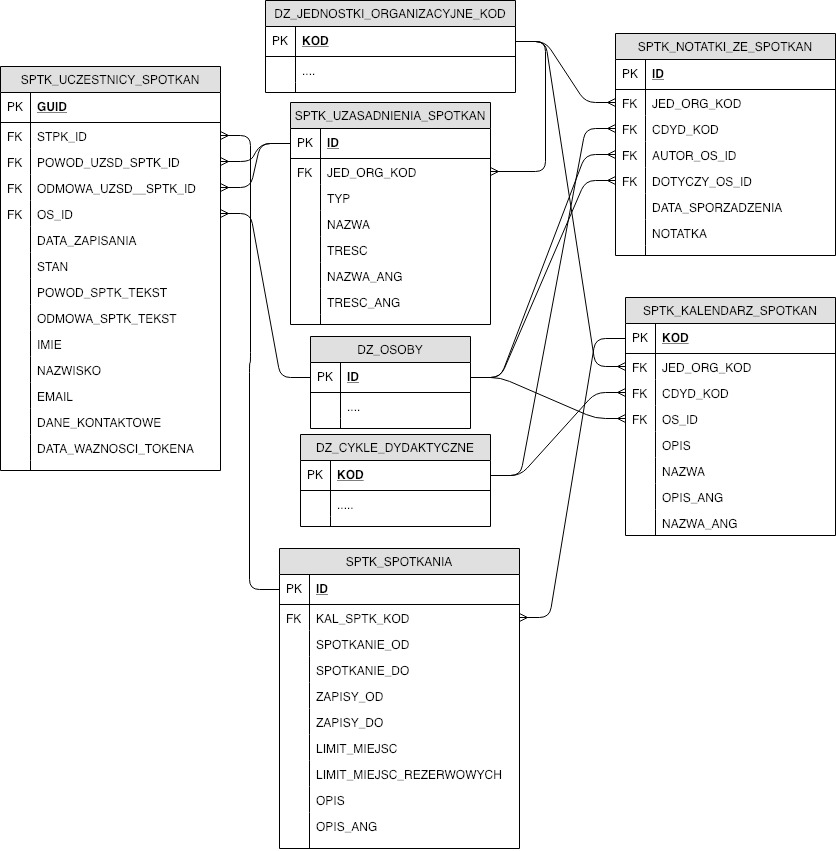
\includegraphics[width=\linewidth]{schemat.jpg}
  \caption{Schemat bazy danych.}
  \label{fig:schemat}
\end{figure}

W wyniku wymagań i potrzeb implementacyjnych, utworzyliśmy następujący schemat bazy danych, pokazany na rysunku \ref{fig:schemat}. Kluczowe jej tabele zawierają następujące informacje:

\begin{itemize}
\item SPTK\textunderscore UCZESTNICY\textunderscore SPOTKAN
	\begin{itemize}
	\item podstawowe dane uczestników spotkania,
	\item id spotkania,
	\item powód wraz z uzasadnieniem,
	\item odmowę wraz z uzasadnieniem,
	\item stan spotkania.
	\end{itemize}
\item SPTK\textunderscore SPOTKANIA
	\begin{itemize}
	\item kalendarz spotkań,
	\item daty spotkania i zapisów,
	\item limit miejsc,
	\item opis.
	\end{itemize}
\item SPTK\textunderscore NOTATKI\textunderscore ZE\textunderscore SPOTKAN
	\begin{itemize}
	\item jednostka organizacyjna,
	\item cykl dydaktyczny,
	\item autor,
	\item osoba której dotyczy,
	\item data utworzenia,
	\item notatka.
	\end{itemize}
\end{itemize}


\section{Przykłady}
Przykładowe scenariusze użycia modułu. Dla prostoty przyjęto dzień jako niepodzielną jednostkę czasu.

%\begin{step}
%	\item Lista rezerwowa
	\setlength{\tabcolsep}{8pt}
	
\begin{table}[h]
	\begin{center}
	\centering
	\caption{Lista Rezerwowa}
	\begin{tabularx}{\textwidth}{ v X n }
	\toprule
	Dzień & Student & Spotkanie1 \\
	\midrule
	1  &    & Definicja \\
	\midrule[0.001em]
	2  & Dostępne spotkania: Spotkanie1.\newline Zapisanie na Spotkanie1, miejsce na~liście rezerwowej. & Zapisy \\
	\midrule[0.001em]
	3  & Kilka miejsc w kolejce zostaje zwolnionych, dostaje się na spotkanie  & Akceptacja \\
	\midrule[0.001em]
	4  &   & Spotkanie \\
	\bottomrule
	\end{tabularx}
	\end{center}
\end{table}
	
%\item Token przeniesienia
\begin{table}[h]
	\begin{center}
	\centering
	\caption{Token przeniesienia}
	\begin{tabularx}{\columnwidth}{ v X n n }
	\toprule
	Dzień & Student & Spotkanie1 & Spotkanie2\\
	\midrule
	1  &    & Definicja & Definicja \\
	\midrule[0.001em]
	2  & Dostępne spotkania: Spotkanie1. \newline Zapisanie na Spotkanie1, miejsce na liście rezerwowej & Zapisy & \\
	\midrule[0.001em]
	3  & Nie dostaje się na spotkanie, pozostaje w rezerwie.  & Akceptacja & \\
	\midrule[0.001em]
	4  & Dostaje token przeniesienia. \newline Dostępne spotkania: Spotkanie2. \newline Przenosi się na Spotkanie2 & Spotkanie & \\
	\midrule[0.001em]
	5  &  &  & Zapisy\\
	\midrule[0.001em]
	6  & Dostaje się na spotkanie &  & Akceptacja\\
	\midrule[0.001em]
	7  &  &  & Spotkanie\\
	\bottomrule
	\end{tabularx}
	\end{center}
\end{table}
	
%\item Token przeniesienia pozwala na przeniesienie tylko do nierozpoczętej rejestracji
\begin{table}[h]
	\begin{center}
	\centering
	\caption{Token przeniesienia pozwala na przeniesienie tylko do nieotwartego spotkania}
	\begin{tabularx}{\columnwidth}{ v X n n n }
	\toprule
	Dzień & Student & Spotkanie1 & Spotkanie2 & Spotkanie3\\
	\midrule
	1  &    & Definicja & Definicja &\\
	\midrule[0.001em]
	2  & Dostępne spotkania: Spotkanie1. \newline Zapisanie na Spotkanie1, miejsce na liście rezerwowej. & Zapisy &  &\\
	\midrule[0.001em]
	3  & Nie dostaje się na spotkanie, pozostaje w rezerwie.  & Akceptacja &  &\\
	\midrule[0.001em]
	4  & Dostaje token przeniesienia.\newline Dostępne spotkania: brak & Spotkanie &  &\\
	\midrule[0.001em]
	5  & Token wygasa &  & Zapisy & Definicja\\
	\midrule[0.001em]
	6  &  &  & Akceptacja & Zapisy\\
	\bottomrule
	\end{tabularx}
	\end{center}
\end{table}
	
	\newpage
%\item Wiele tur jednocześnie
\begin{table}[h]
	\begin{center}
	\centering
	\caption{Wiele tur jednocześnie}
	\begin{tabularx}{\columnwidth}{ v X m m }
	\toprule
	Dzień & Student & Spotkanie1 & Spotkanie2 \\
	\midrule
	1  &    & Definicja & Definicja \\
	\midrule[0.001em]
	2  & Dostępne spotkania: Spotkanie1. \newline Zapisanie na Spotkanie1, miejsce na liście rezerwowej. & Zapisy & Zapisy\\
	\midrule[0.001em]
	3  & Nie dostaje się na spotkanie, pozostaje w rezerwie.  & Akceptacja & Zapisy\\
	\midrule[0.001em]
	4  & Dostaje token przeniesienia.\newline Dostępne spotkania: brak.\newline Dostępne spotkania: Spotkanie2.\newline Zapisanie na Spotkanie2 & Spotkanie & Zapisy\\
	\midrule[0.001em]
	5  & Token wygasa &  & Akceptacja \\
	\midrule[0.001em]
	6  &  &  & Spotkanie \\
	\bottomrule
	
	\end{tabularx}
	\end{center}
\end{table}
%\end{step}

\chapter{Implementacja} \label{chap:implementacja}
\section{USOS}
USOS jest skomplikowanym systemem, rozwijanym przez lata. Składa się on obecnie z wielu komponentów odpowiadających za różne zbiory funkcjonalności potrzebnych do obsługi studiów. Ze względu na zróżnicowane okresy powstawania oraz przeznaczenie, różnią się między sobą znacząco technologią wykonania, a zasada współdziałania całego systemu jest bardzo skomplikowana.
Składowe, z którymi mieliśmy styczność podczas naszej pracy, to:
\begin{itemize}
\item USOSadm w Javie -- moduł przeznaczony dla pracowników administracji,
\item USOSweb -- moduł przeznaczony dla studentów,
\item baza danych Oracle -- centralna baza danych USOS, posiada bogatą wewnętrzną logikę odpowiadającą między innymi za dostęp do danych, bezpośrednio kontaktuje się z nią USOSadm,
\item baza danych MySQL -- baza danych z którą łączy się USOSweb, w większości kopia bazy danych Oracle,
\item Migrator -- moduł odpowiedzialny za synchronizację baz danych, ponieważ ruch w systemie USOS jest rozproszony pomiędzy wiele modułów i baz danych, Migrator dba o zachowanie spójności danych z centralną bazą wykonując częste, okresowe migracje.
\end{itemize}

\section{USOSadm} \label{sec:impusos}

\subsection{Informacje ogólne}
Celem prac w obrębie USOSadm było zaimplementowanie funkcjonalności przy wykorzystaniu przyjętych praktyk programistycznych. Jej zakres obejmował następujące mechanizmy:
\begin{itemize}
\item definiowania nowych kalendarzy spotkań oraz spotkań z pracownikami uczelni,
\item zapisu i akceptowania zapisów na spotkania studentów,
\item sporządzania notatek ze spotkań,
\item definiowania listy najczęstszych powodów zapisów na spotkania,
\item mechanizm tokenowy, pozwalający odrzuconym studentom zapisać się na kolejne spotkanie z uprzywilejowaną pozycją.
\end{itemize}

\subsection{Aplikacja kliencka}
Aplikacja kliencka USOSadm to część aplikacji wykonywana po stronie klienta. Składa się m.in. z~kodu HTML i~skryptów JavaScript. Napisana została przy pomocy frameworka JavaServer Faces z wykorzystaniem biblioteki komponentów RichFaces.

\subsection{Serwer}
Serwer USOSadm odpowiedzialny jest za~większą część logiki aplikacji. Napisany został w Javie. Część logiki wykonywana jest po~stronie~bazy~danych~Oracle.

\subsection{Komunikacja z bazą danych}
Komunikacja z~bazą~danych została zrealizowana przy pomocy własnego, bogatego API zrealizowanego przy pomocy technologi Hibernate. Technologia Hibernate pozwala na~odwzorowanie danych z~bazy~danych za~pomocą odpowiednio spreparowanych obiektów w~Javie.

\subsection{Opis implementacji}
Funkcjonalność została wydzielona w oddzielnym module do USOSadm, \enquote{Spotkania}. Składa się łącznie z 4 widoków:
\begin{itemize}
\item Słownik uzasadnień -- pozwala zdefiniować najczęstsze uzasadnienia zapisów na spotkania jak i odrzucenia spotkań.
\item Kalendarz Spotkań -- pozwala na definicję kalendarzy spotkań, spotkań, zapisywanie studentów oraz akceptowanie zapisów na spotkania.
\item Notatki -- pozwala na przeglądanie i dodawanie notatek ze spotkań osób.

\subsection{Słownik uzasadnień}
Widok Słownika Uzasadnień jest bardzo prosty w budowie i obsłudze.

\begin{figure}[b!]
  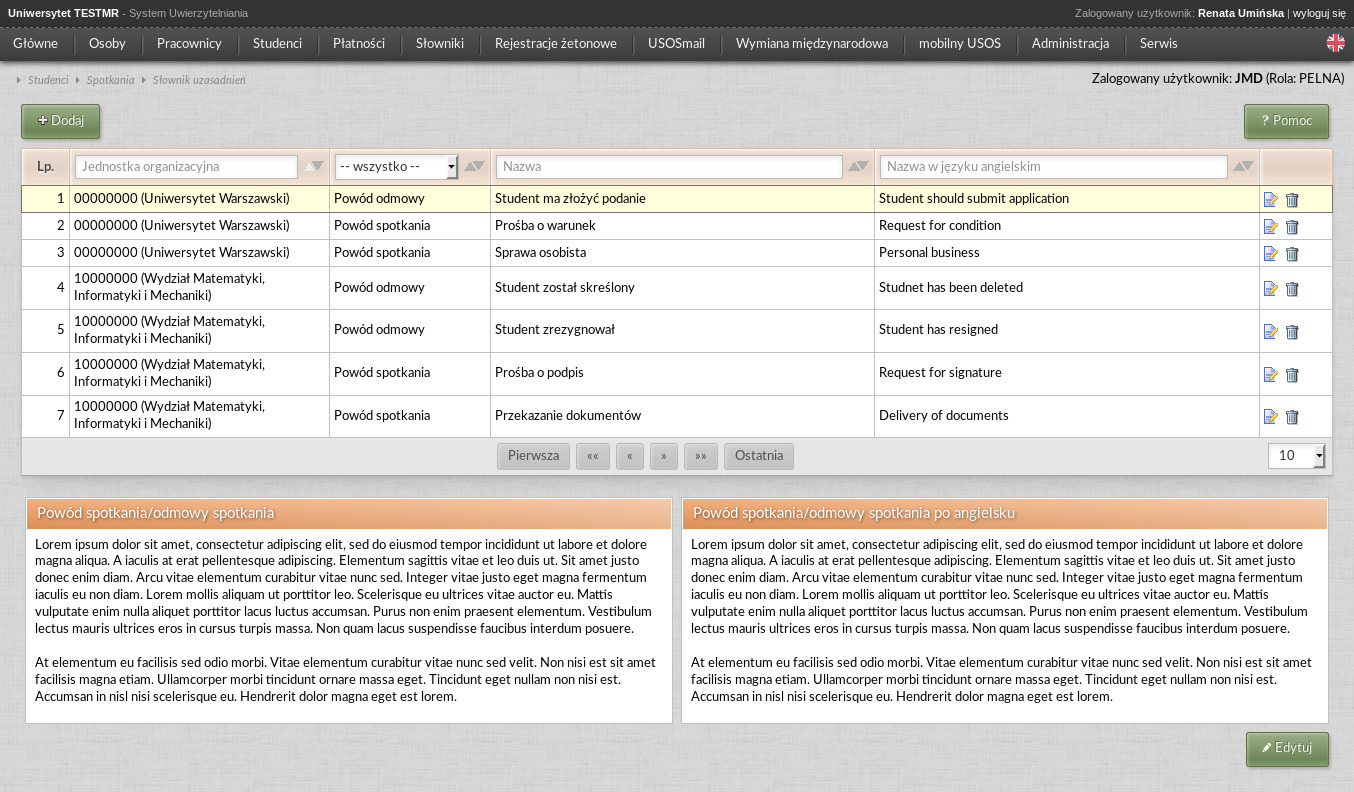
\includegraphics[width=\linewidth]{widok_uzasadnien.jpg}
  \caption{Widok uzasadnień zapisów na spotkanie.}
  \label{fig:uzasadnienia}
\end{figure}

\begin{figure}[b!]
  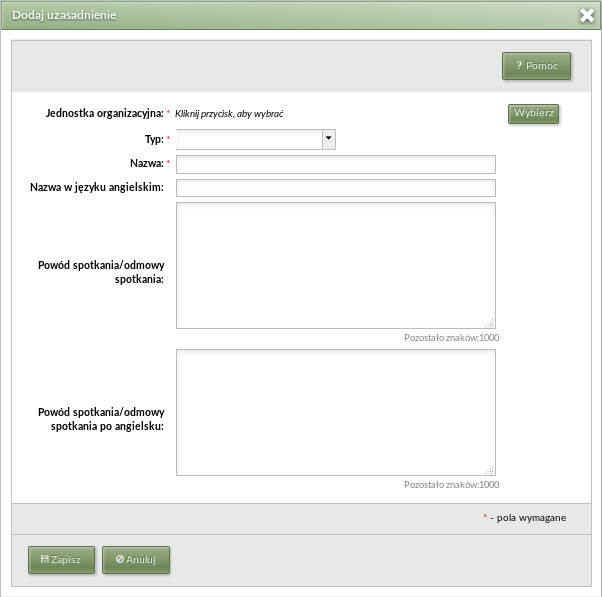
\includegraphics[width=\linewidth]{formularz_uzasadnien.jpg}
  \caption{Formularz dodawania uzasadnienia zapisu na spotkanie.}
  \label{fig:formularz_uzasadnienia}
\end{figure}

\subsection{Kalendarz}
TODO: Wstawić screena i napisać co trzeba klikać

\subsection{Notatki}
Widok notatek w sumie też.

\begin{figure}[b!]
  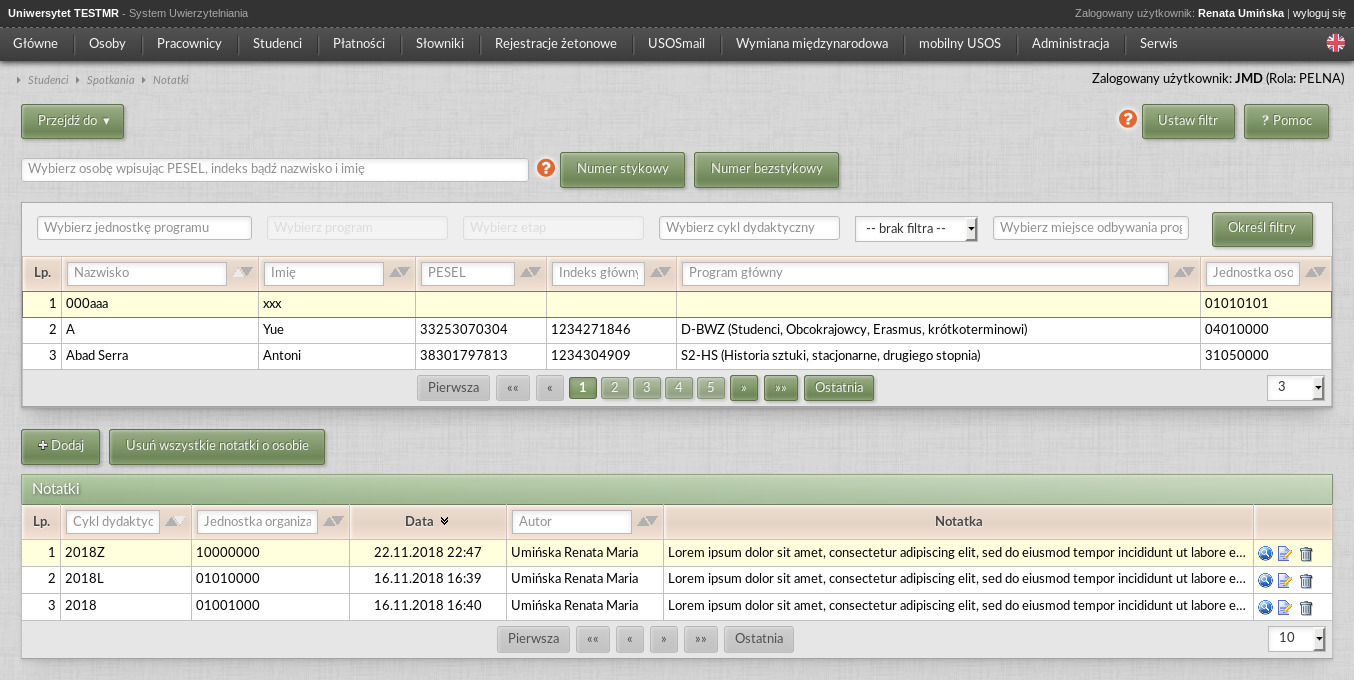
\includegraphics[width=\linewidth]{widok_notatek.jpg}
  \caption{Widok notatek ze spotkań.}
  \label{fig:notatki}
\end{figure}

\begin{figure}[b!]
  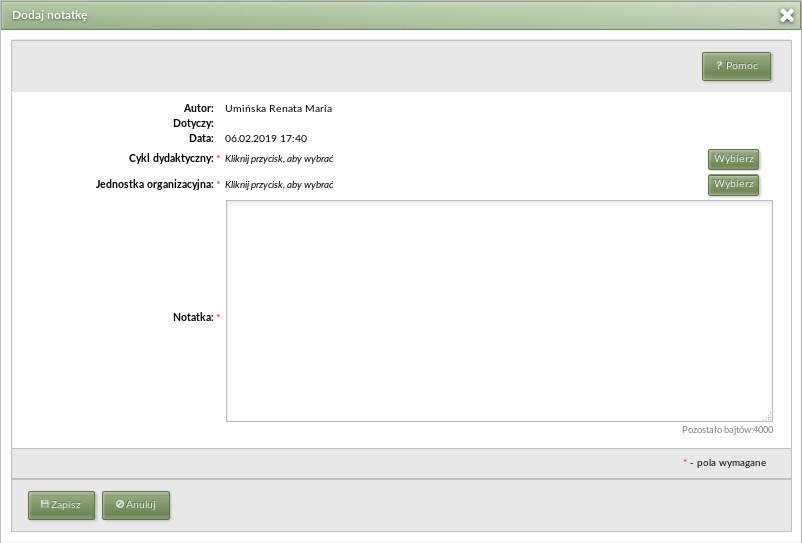
\includegraphics[width=\linewidth]{formularz_notatek.jpg}
  \caption{Formularz dodawania notatki ze spotkania.}
  \label{fig:formularz_notatek}
\end{figure}



\section{USOSweb}\label{sec:impusosweb}
Implementacja funkcjonalności w USOSweb polega na rozbudowaniu go, używając najlepszych w danej chwili praktyk programowania przyjętych przez zespół tworzący USOSweb. Zachowując spójność z pozostałym kodem systemu, stworzyliśmy moduł pozwalający studentowi na:
\begin{itemize}
\item{wybór jednostki w ramach której odbywa się interesujące studenta spotkanie,}
\item{wyświetlanie kalendarza spotkań wybranej osoby lub jednostki,}
\item{wyświetlanie terminów spotkań dla każdego kalendarza,}
\item{wykonywanie dostępnych akcji związanych ze spotkaniem:
\begin{itemize}
\item{zapisywanie się na listę główną lub rezerwową,}
\item{wypisywanie się,}
\item{podgląd aktualnego stanu zapisu na spotkanie, w tym informacje takie jak liczba dostępnych miejsc,}
\end{itemize}
}
\item{wyświetlanie spotkań związanych ze studentem.}
\end{itemize}

Dużą uwagę zwróciliśmy na uniemożliwienie studentowi wykonywania akcji, do których w danej chwili nie ma on dostępu. W tym celu przy każdym zapytaniu do serwera, które powodowałoby zmianę w bazie danych - sprawdzamy czy dany student ma dostęp do tej akcji. Moduł został zabezpieczony przeciwko potencjalnym atakom. Więcej na ten temat w sekcji \ref{subsec:bezpiecz}.
\subsection{Opis działania systemu USOSweb}
USOSweb oparty jest o kontroler zaimplementowany w języku PHP, który dostaje w parametrach GET opis akcji, jaką użytkownik chciałby wykonać. Każda akcja zaimplementowana jest jako osobna klasa języka PHP (akcja obsługuję całą logikę, ona tworzy wynikowe dane i ewentualnie powoduje efekty uboczne). Za pomocą plików konfiguracyjnych actions.xml akcje wiążą się z szablonami (szablony odpowiadają za format wyświetlania danych, które są wynikiem akcji). Akcje mogą, a czasami muszą, korzystać z dodatkowych modułów, które tworzymy jako osobne statyczne albo niestatyczne klasy.

\subsection{Akcje}
Podczas implementacji przez nas modułu spotkań, powstało pięć akcji.
\begin{itemize}
\item{MojeSpotkaniaAction
\subitem{akcja odpowiada za wyświetlanie spotkań, związanych z zalogowanym studentem.}
}
\item{SpotkaniaJednostkiAction
\subitem{akcja odpowiada za wyświetlanie kalendarzy spotkań wraz z terminami tych spotkań oraz związanych z nimi informacji w wybranej jednostce.}}
\item{WyborJednostkiAction
\subitem{akcja odpowiada za wyświetlanie jednostek i informacji o ilości spotkań w każdej z jednostek. Przyjmuje dodatkowy parametr w GET, który włącza lub ~wyłącza ograniczenie listy jednostek tylko do tych, które są związane ze~studentem.}}
\item{ZapisNaSpotkanieAction
\subitem{akcja odpowiada za tworzenie formularza, pozwalającego na wykonywanie przez studenta dostępnych działań z~danym~spotkaniem. Akcja przyjmuje w GET informację o~spotkaniu, czyli identyfikator spotkania z bazy i tworzy odpowiedni formularz dla studenta w~zależności od tego, co zalogowany student może zrobić ze~wskazanym~spotkaniem w~danym~momencie.}}
\item{ZmianaZapisuNaSpotkanieAction
\subitem{akcja odpowiada za~zmianę stanu zapisu zalogowanego studenta na dane spotkanie. Jest to jedyna akcja w~danym module, która zmienia dane w~bazie danych. Przyjmuje ona parametry zapytania w postaci POST i~sprawdza CSRF token w celu zabezpieczenia się przed atakami CSRF. Dla każdego zapytania przed modyfikowaniem danych w bazie na początku jest prowadzony proces tak zwanej walidacji w~celu uniemożliwienia wykonania niepoprawnych zmian.}}
\end{itemize}
\subsection{Szablony}
USOSweb korzysta z szablonów smarty, które są powiązane z~akcjami za~pomocą plików konfiguracyjnych i~zapewniają odpowiednią prezentację danych powstających w~wyniku danej akcji. W~module~spotkań utworzyliśmy pięć szablonów.
\begin{itemize}
\item{FormularzSpotkania}
\subitem{formularz, który wyświetla się w~oknie~modalnym i pozwala na wykonanie przez studenta dozwolonej akcji związanej ze spotkaniem.}
\item{SpotkaniaJednostki}
\subitem{rozwijana lista cykli, gdzie domyślnie rozwinięte są tylko aktywne cykle. Każdy cykl zawiera listę kalendarzy spotkań. Dla każdego kalendarza wyświetlany zostaje opis osoby prowadzącej spotkania i nazwa kalendarza spotkań. Zawiera on również listę dostępnych terminów i~przycisk pozwalający na pokazanie także niedostępnych terminów.}
\item{MojeSpotkania}
\subitem{lista spotkań związanych ze studentem. Widok jest identyczny z~widokiem spotkań jednostki, ale pokazywane są tylko spotkania i~kalendarze związane z danym studentem, czyli takie, na które on jest albo był zapisany. Nie ma żadnych ograniczeń na jednostkę w której dane spotkanie się odbywa.}
\item{Spotkanie}
\subitem{szablon pomocniczy używany w szablonie FormularzSpotkania.}
\item{WyborJednostki}
\subitem{lista jednostek z informacją o ilości spotkań w danej jednostce.}
\end{itemize}
\subsection{Moduły pomocnicze}
Często akcje w USOSweb wykonują te same czynności jak pobranie kontekstu zalogowanego użytkownika lub nazwy jednostki na podstawie kodu, albo utworzenie struktury pozwalającej na wyświetlanie tabeli z~danymi na~podstawie zapytania.
W naszym rozwiązaniu zostały utworzone cztery moduły pomocnicze.
\begin{itemize}
\item{CyklDydaktyczny}
\subitem{klasa jest modelem cyklu dydaktycznego. Zawiera jedną statyczną metodę pozwalającą na pobranie z~bazy danych informacji o~wszystkich kalendarzach spotkań w cyklu dla danej jednostki wraz z terminami spotkań i~kontekstem każdego osobnego spotkania dla~użytkownika. Funkcja ta korzysta ze~stałej~liczby zapytań do~bazy~danych.}
\item{KalendarzSpotkan}
\subitem{klasa jest modelem Kalendarza Spotkań i~posiada metodę statyczną, pozwalającą na~pobranie z~bazy~danych informacji o~wszystkich kalendarzach spotkań i~spotkaniach dla każdego z~kalendarzy. wykonuje 2 zapytania do bazy danych.}
\item{SpotkanieOsoba}
\subitem{klasa jest modelem opisującym stan spotkania w~kontekście danej osoby. Ma dużą ilość niestatycznych funkcji pomocniczych, wykorzystywanych w wielu miejscach modułu spotkań.}
\item{SpotkaniaUtils}
\subitem{zestaw funkcji pomocniczych.}
\end{itemize}

\subsection{Wybór jednostki}
TODO: Wstawić screena i napisać co trzeba klikać (Może to wywalić?)

\subsection{Wybór spotkania}

\begin{figure}[b!]
  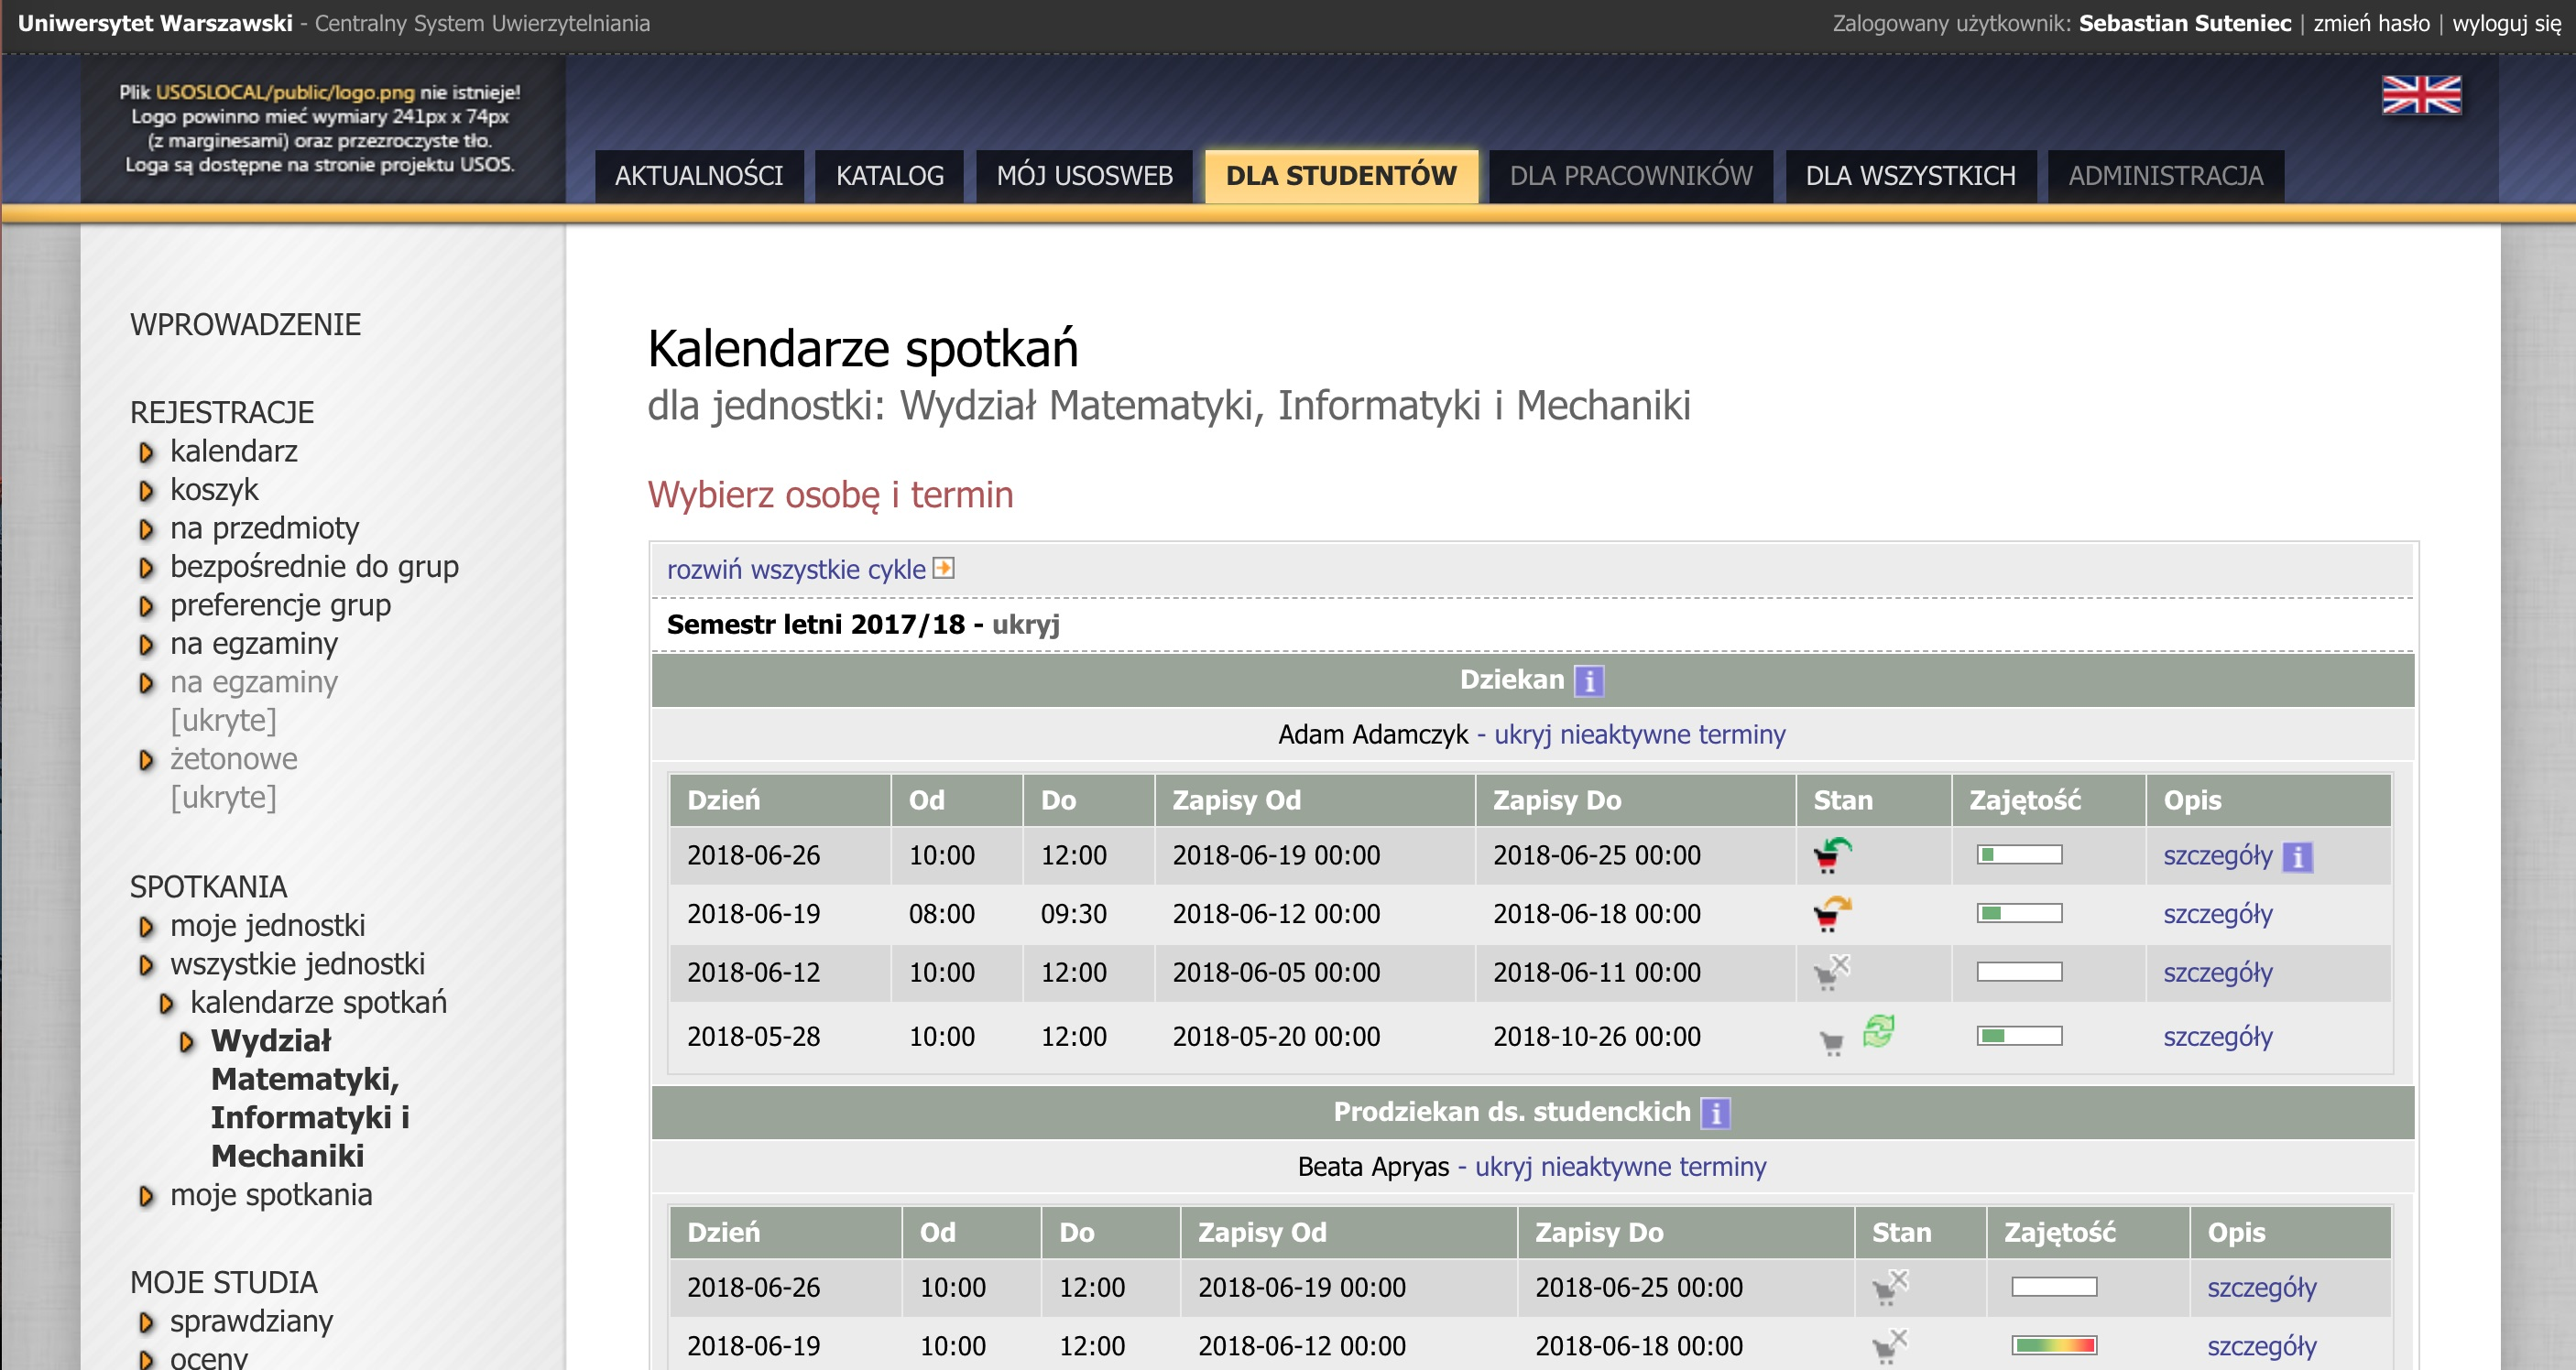
\includegraphics[width=\linewidth]{kalendarzUSOSweb.jpg}
  \caption{Kalendarz spotkań.}
  \label{fig:kalweb}
\end{figure}

Na ekranie \ref{fig:kalweb} są widoczne trzy kalendarze spotkań. Jeden z nich nie ma zdefiniowanego żadnego spotkania. Pozostałe dwa mają po jednym spotkaniu, na które można się zapisać. Aby zapisać się należy kliknąć odpowiedni przycisk.

\begin{figure}[b!]
  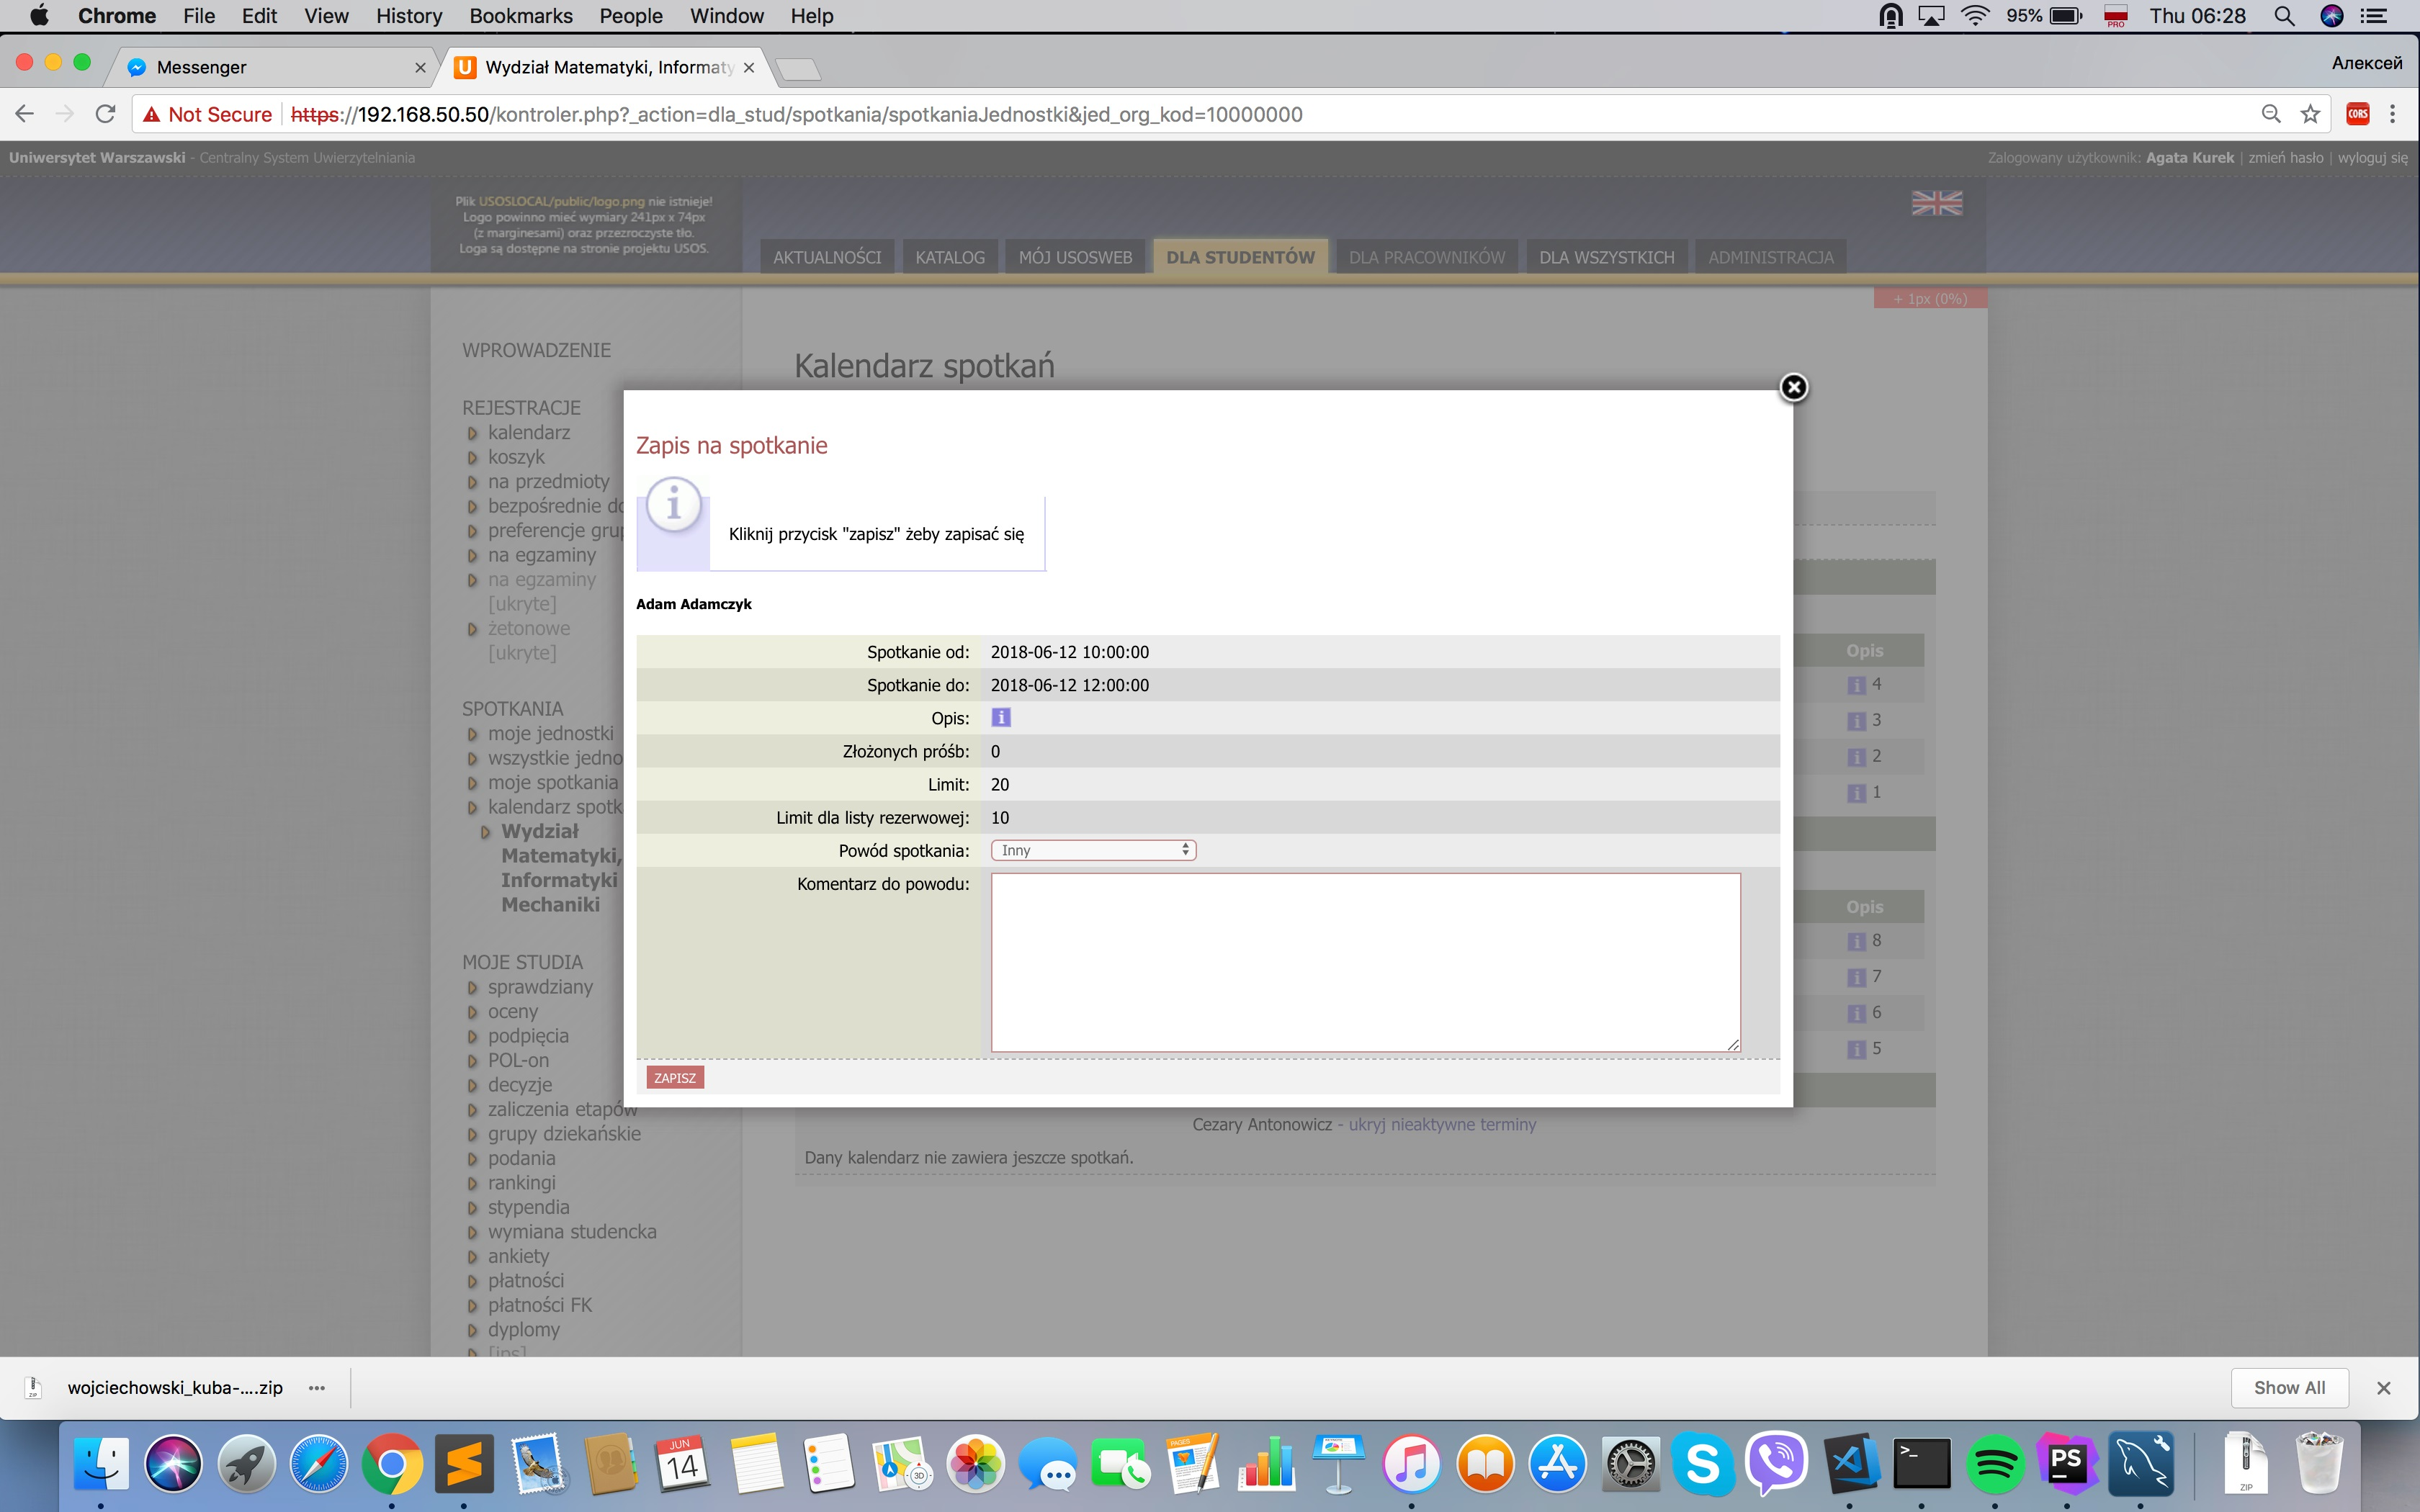
\includegraphics[width=\linewidth]{zapisUSOSweb.jpg}
  \caption{Zapis na spotkanie.}
  \label{fig:zapisweb}
\end{figure}

Ekran \ref{fig:zapisweb}: Należy wybrać powód zapisu z listy, dodać komentarz tekstowy i kliknąć przycisk \enquote{ZAPISZ}.

\subsection{Moje spotkania}

\begin{figure}[b!]
  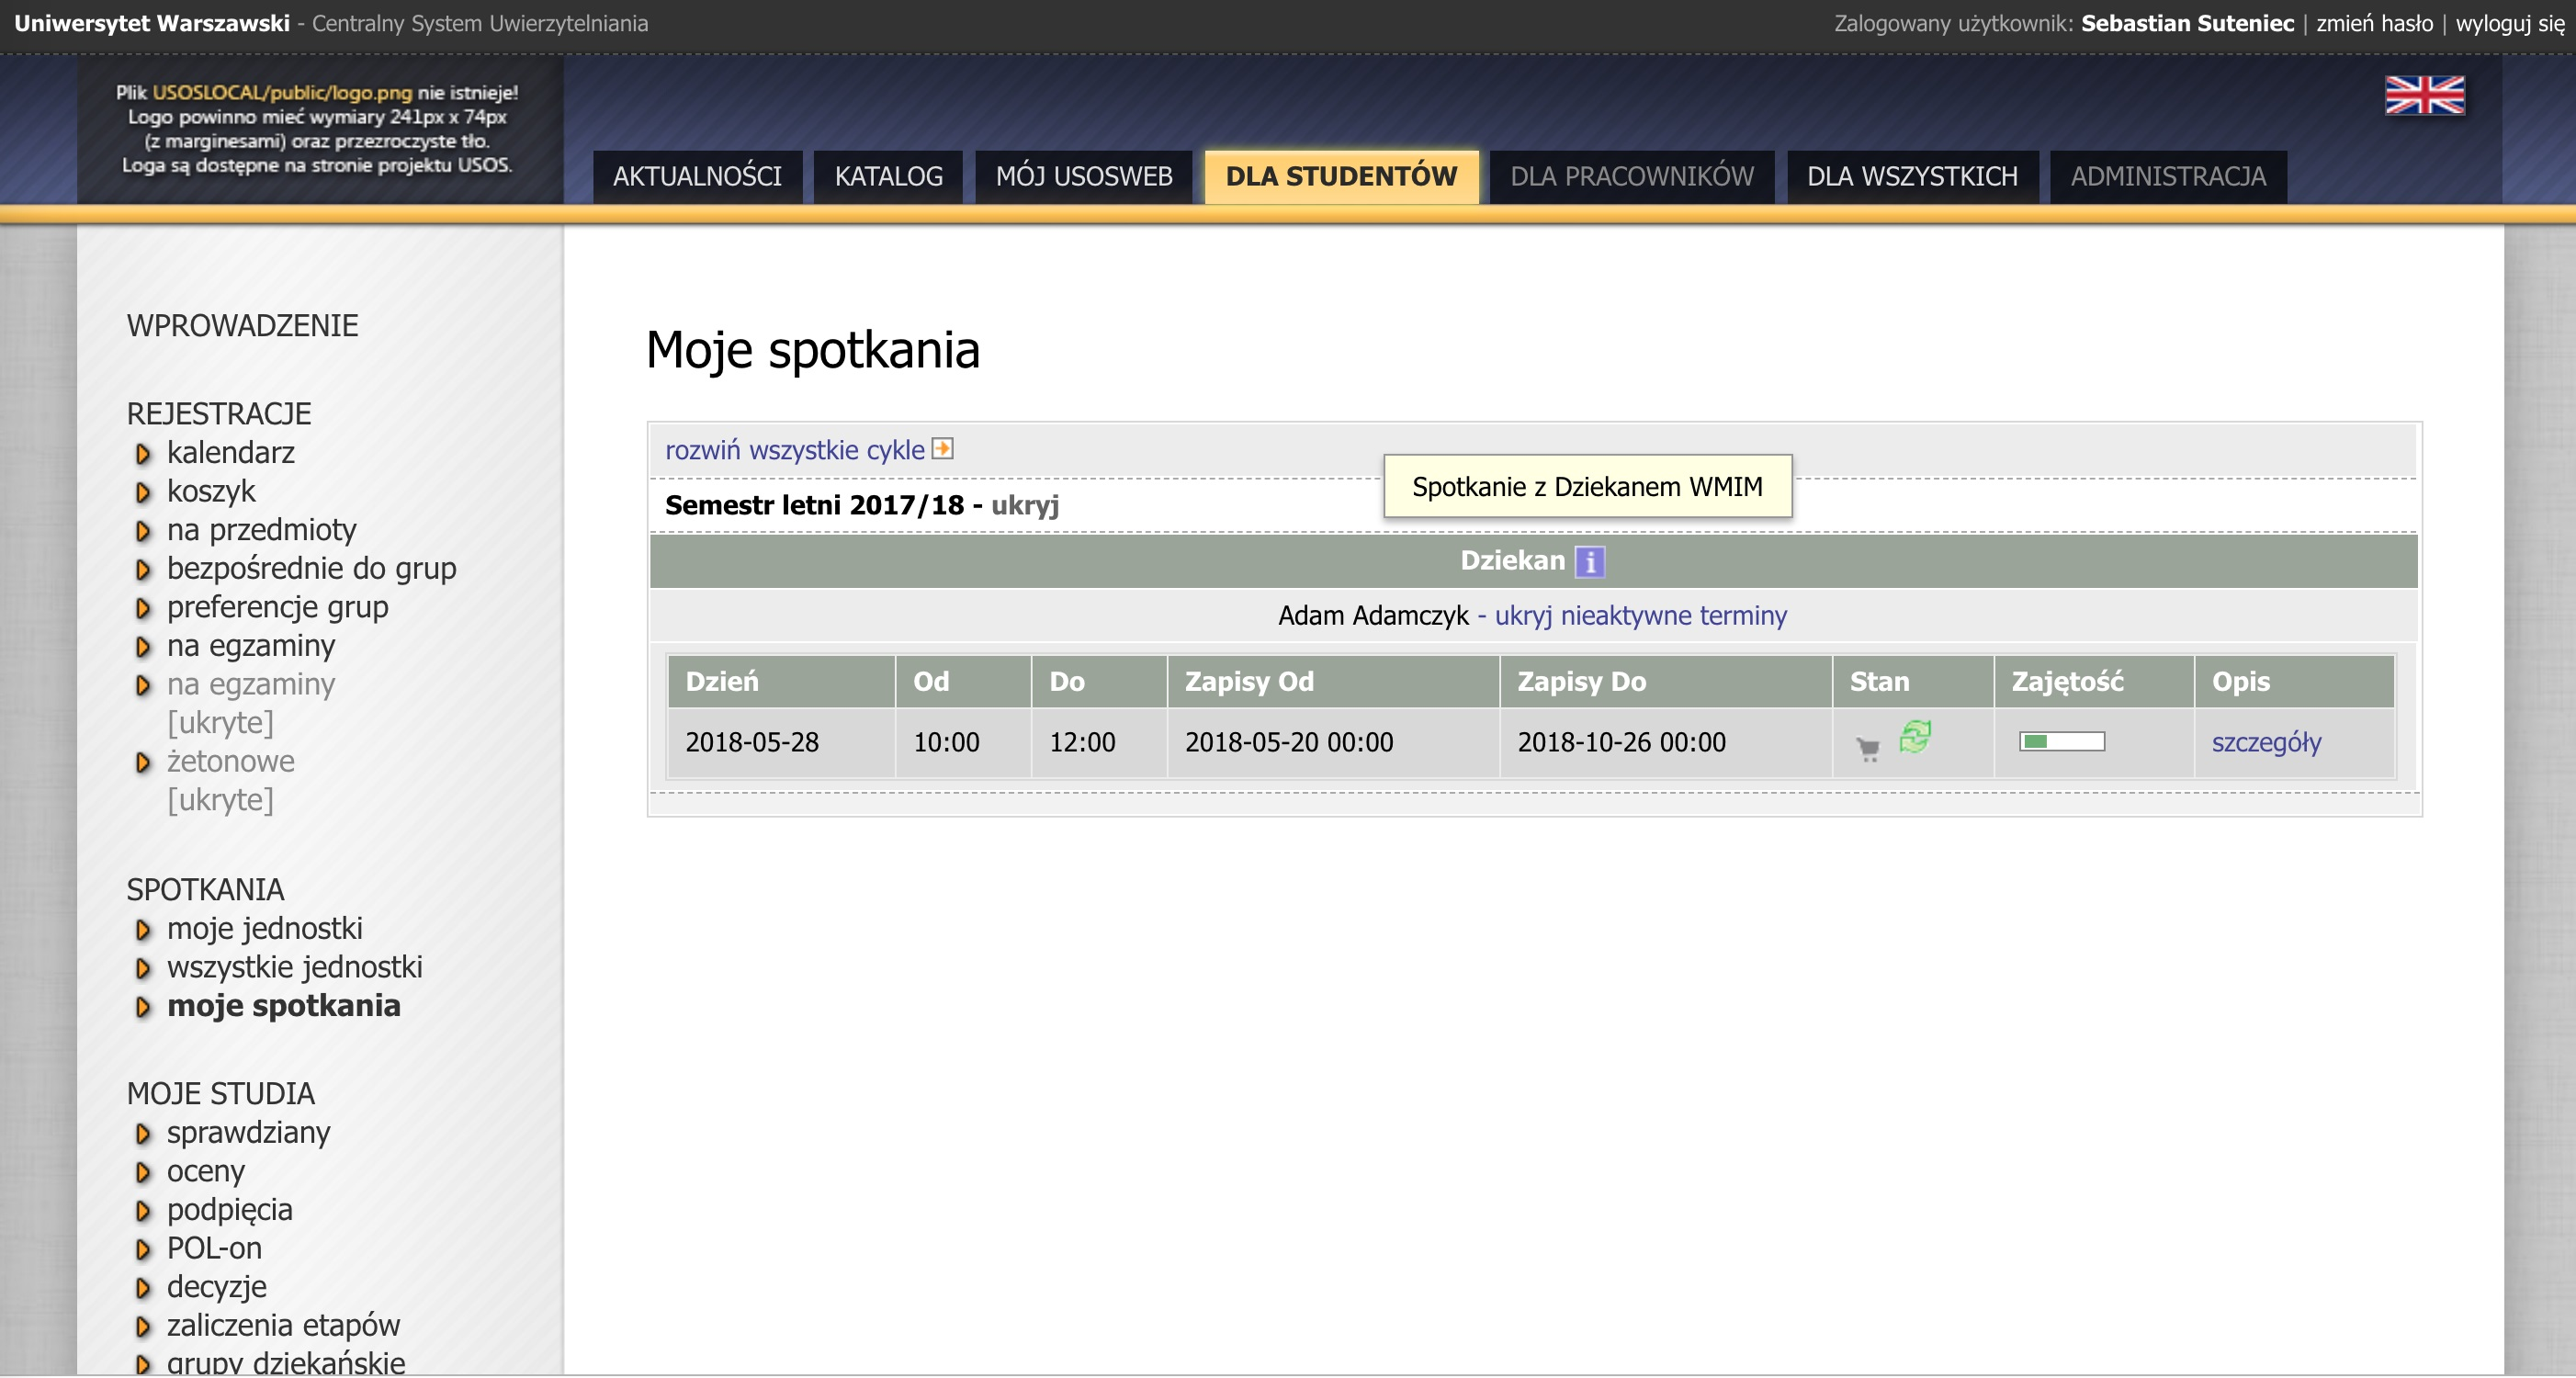
\includegraphics[width=\linewidth]{mojeSpotkaniaUSOSweb.jpg}
  \caption{Moje spotkania.}
  \label{fig:mojeweb}
\end{figure}

Na ekranie \ref{fig:mojeweb} widać spotkania, na które student złożył prośbę o zapisanie. Można sprawdzić, czy prośba została zaakceptowana.

\subsection{Problemy i ich rozwiązania}
\subsubsection{Pobranie nietypowej drzewiastej struktury z danymi o spotkaniach}
Widok spotkań danej jednostki oraz widok spotkań studenta został zaprojektowany w taki sposób, że do jego realizacji potrzebowaliśmy dostać w wyniku akcji drzewiastą strukturę następnej postaci:

\begin{itemize}
\item{pierwszy poziom}
\subitem{cykle dydaktyczne z informacją pomocniczą (nazwa, stan, kod),}
\item{drugim poziom}
\subitem{kalendarze spotkań, gdzie każdy kalendarz wskazuje na odpowiedni cykl dydaktyczny, oraz informacje z nimi związane (nazwa, osoba),}
\item{trzeci poziom}
\subitem{spotkania (terminy) z informacją o stanie danego spotkania w kontekście zalogowanego studenta (stan zapisu, stan spotkania, ilość osób zapisanych na~listę~główną oraz~rezerwową, data i~czas rozpoczęcia i~zakończenia spotkania i tym podobne).}
\end{itemize}
Używając instrumentów językowych dostępnych w PHP taką strukturę najwygodniej przedstawić jako listę obiektów cykli, gdzie każdy z~nich ma pole \enquote{kalendarzeSpotkan}, będące listą obiektów kalendarzy spotkań w danym cyklu. Każdy z tych obiektów miałby pole spotkania, będące listą obiektów klasy \enquote{SpotkanieOsoba} i~zawierał całą informację pomocniczą. 
Zastanawialiśmy się w jaki sposób wyciągnąć taką drzewiastą strukturę z bazy danych w optymalny sposób. Relacyjne bazy danych SQL pozwalają na pobranie informacji w~postaci tabel. Można by pobierać listę cykli, potem dla każdego cyklu listę kalendarzy i~dla~każdego~kalendarza listę spotkań. Co prawda, to spowodowałoby gigantyczną ilość zapytań. Innym rozwiązaniem mogło być pobranie całej drzewiastej struktury w jednym zapytaniu. Ponieważ relacyjna baza danych z której korzystamy zwraca dane tylko w postaci tabel można wywnioskować, że pobieralibyśmy gigantyczną ilość zbędnych i~duplikujących się danych o cyklach i~kalendarzach. Wybranym przez nas rozwiązaniem było wykonanie trzech zapytań: pobieranie cykli i~informacji o~nich, pobieranie kalendarzy wraz z~informacjami o~nich oraz~pobranie~spotkań. Po pobraniu danych wiążemy je: tworzymy opisaną wyżej drzewiastą strukturę, iterując po każdej z~list i~używając informacji zawartej w~polach z~kodem cyklu albo~kodem~kalendarza.

\subsubsection{Podobne akcje}
W module spotkań mieliśmy dwie pary bardzo podobnych akcji: akcje spotkań studenta i~spotkań w~jednostce oraz~akcje wyświetlania jednostek użytkownika i~akcje wyświetlania wszystkich jednostek. W przypadku każdej z~tych par utworzyliśmy implementację ich wspólnej części i~korzystaliśmy z~niej, zapobiegając duplikowania kodu.
\subsubsection{Wielojęzyczność}
System USOSweb wspiera dwa języki: angielski oraz polski. Dla wsparcia wielojęzyczności w naszym module korzystaliśmy z wbudowanego w szablony smarty znacznika \{t\}, a w~modelu bazy danych dla pól tekstowych takich jak nazwa albo opis tworzyliśmy duplikat w języku angielskim.
\subsection{Zmiany w USOSWebie}
\subsubsection{Wyjątki}
Przy wysyłaniu danych do serwera w postaci JSON chcieliśmy otrzymać informację o~ewentualnym~błędzie również w postaci JSON. W tym celu rozbudowaliśmy mechanizm wyjątków używany w USOSweb dodając możliwość zwracania wyniku wyjątku w postaci JSON wskazując odpowiednią opcję w momencie podnoszenia wyjątku, który jest obiektem klasy ActionError.
\subsubsection{Błąd w smarty}
W trakcie implementowania natknęliśmy się na~błąd w~implementacji znacznika \{textarea\} w~szablonach~smarty. Po wskazaniu atrybutu \enquote{limit} w~danym~tagu, będąc w~kontekście okna modalnego cała zawartość strony znikała. Zmieniliśmy kod JavaScript obsługujący wypisywanie limitu oraz pozostałych dostępnych liter, naprawiając ten błąd.
\subsection{Potencjalne ataki i zabezpieczenia} \label{subsec:bezpiecz}
\subsubsection{CSRF}
W celu zapobiegania potencjalnym atakom CSRF w jedynym miejscu w którym zmieniamy dane dodaliśmy sprawdzenie tokenu CSRF.
\paragraph{SQL injection}
Każdy parametr będący częścią zapytania do bazy jest escape-owany w celu zapobiegania atakom typu SQL-injection.

%\chapter{Dokumentacje użytkownika} \label{chap:dokumentacja_uzytkownika}
%\section{Dokumentacja USOS}
%\section{Dokumentacja USOSweb}

%\chapter{Dokumentacja instalacyjna} \label{chap:dokumentacja_instlacyjna}

%\chapter{Opis zawartości płytki CD} \label{chap:opis_plytki}

\chapter{Potencjalny dalszy rozwój}  \label{chap:rozwoj}

\section{Mobilny USOS}

W ankiecie dla studentów pojawiły się odpowiedzi, że studenci chcieliby znać godzinę spotkania, a nie tylko numer na liście. Projekt będzie można rozszerzyć o integracje z mobilnym USOS. Potrzebne będzie stworzenie mechanizmów do kontroli stanu spotkania i przepływu studentów w czasie rzeczywistym. Dodanie akcji Dziekana, w której określałby, które spotkanie się rozpoczęło/zakończyło oraz odpowiednich funkcji w mobilny USOS mogłoby umożliwić śledzenie stanu spotkania przez studentów. Na przykład student jest na zajęciach, sprawdza przebieg spotkania w aplikacji mobilnej i wie, w którym momencie musi iść na spotkanie.

\section{Spotkania innego rodzaju}
W rozdziale~\ref{chap:wpr} zauważono, że system powstał po to, aby prowadzić zapisy na spotkania z Dziekanem MIM. Dalszy rozwój systemu mógłby dopasować system również do organizacji innych wydarzeń. Wymagałoby to możliwości obsługi spotkań poprzez pracowników naukowych z poziomu USOSweb. Możliwe byłoby tworzenie wydarzeń takich jak:
\begin{itemize}
	\item konsultacje z dydaktykami,
	\item spotkania studenckie lub okolicznościowe np. święta Bożego Narodzenia.
\end{itemize}

%\chapter{Spis literatury}
\chapter{Dodatki} \label{chap:dodatki}
%\section{Dokumentacja USOS}
%\section{Dokumentacja USOSweb}
%\section{Dokumentacja instalacyjna}
\section{Opis zawartości płyty CD}
TODO

\begin{thebibliography}{99}
\addcontentsline{toc}{chapter}{Bibliografia}

\bibitem[przewodnik]{prz} Jan Rudziński, \textit{Przewodnik po systemie}, Między uniwersyteckie Centrum Informatyzacji, 2010, https://www.usos.edu.pl/sites/default/files/pl-usos-przewodnik.pdf.


\end{thebibliography}

\end{document}


%%% Local Variables:
%%% mode: latex
%%% TeX-master: t
%%% coding: latin-2
%%% End:
